\section{Scalability GAMYGDALA}
The developers of GAMYGDALA choose to not implement some of the Software Engineering Method, because most of the time it will impact the scalability of the code.
But the port of GAMYGDALA has been refactored and some Software Engineering Methods has been applied. So the GAMYGDALA port had to be tested if the refactor has impact on the scalability. \\

We tested GAMYGDALA by calculating the execution time of the \texttt{appraise()} and the \texttt{decayAll()}. This because those two methods are affected by the amount of entities with in engine. Because are so many entities within GAMYGDALA the test has been split into three smaller once which are different in the amount of relation between Agents, the amount of Beliefs that have to be appraised and the amount of Goals that are affected by the Beliefs.

Foreach test the duration had been calculated for 1, 10, 100, 1000 and 10000 Agents with 5, 50 and 500 Goals per Agent. Below you can see the result of the test plotted into three different graph. Below each graph you can see the settings of the test. The x and y-axis are logarithmic.

\begin{figure}[H]
  \centering
  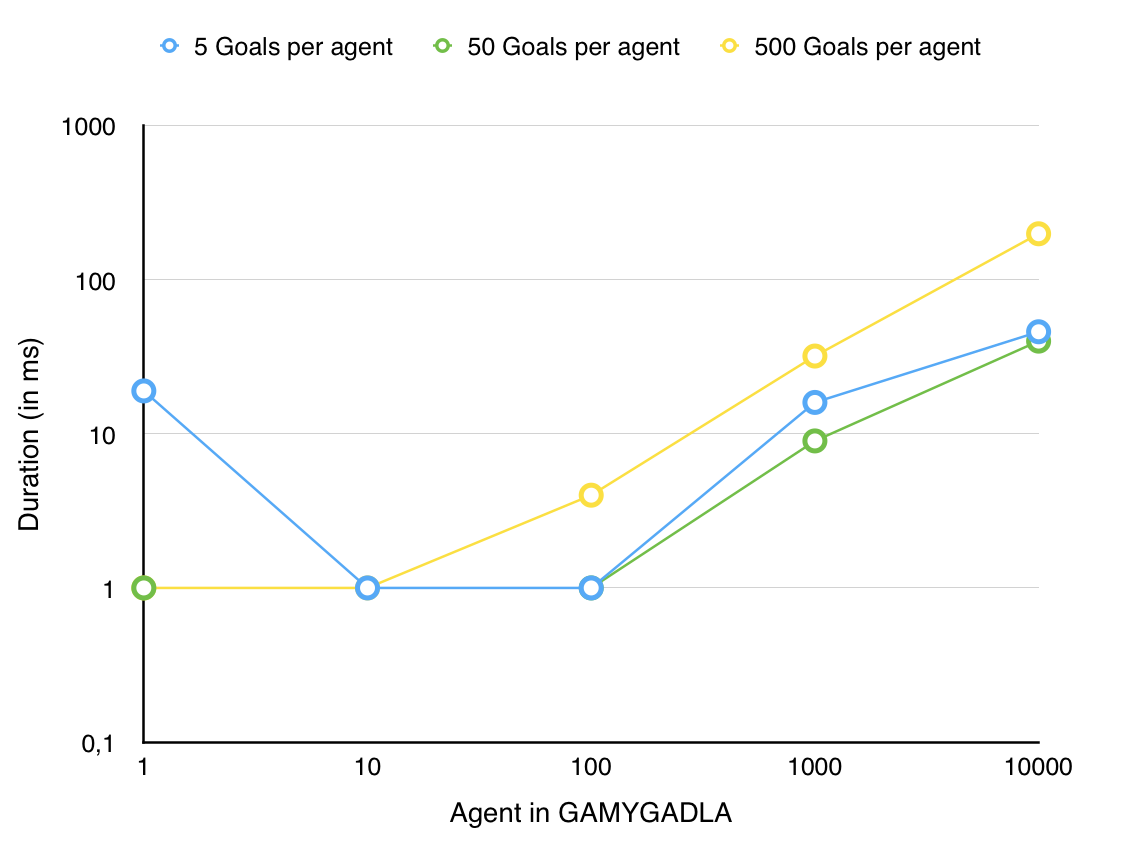
\includegraphics[scale=0.5]{scalability/1.jpg}
  \caption{Scalability, Relation: 1, Belief: 1 and Affected Goals: 1}
  \label{scala:first}
\end{figure}

\begin{figure}[H]
  \centering
  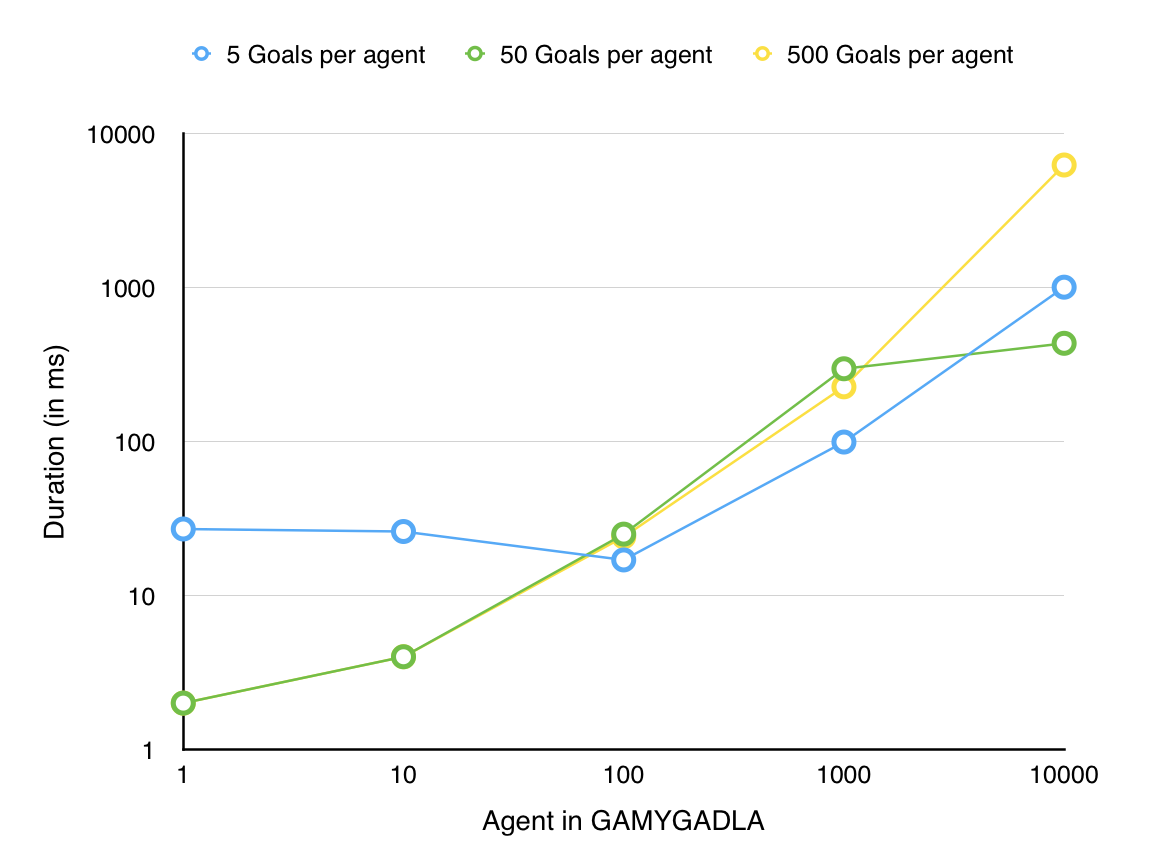
\includegraphics[scale=0.5]{scalability/2.jpg}
  \caption{Scalability, Relation: 10, Belief: 10 and Affected Goals: 10}
  \label{scala:second}
\end{figure}

\begin{figure}[H]
  \centering
  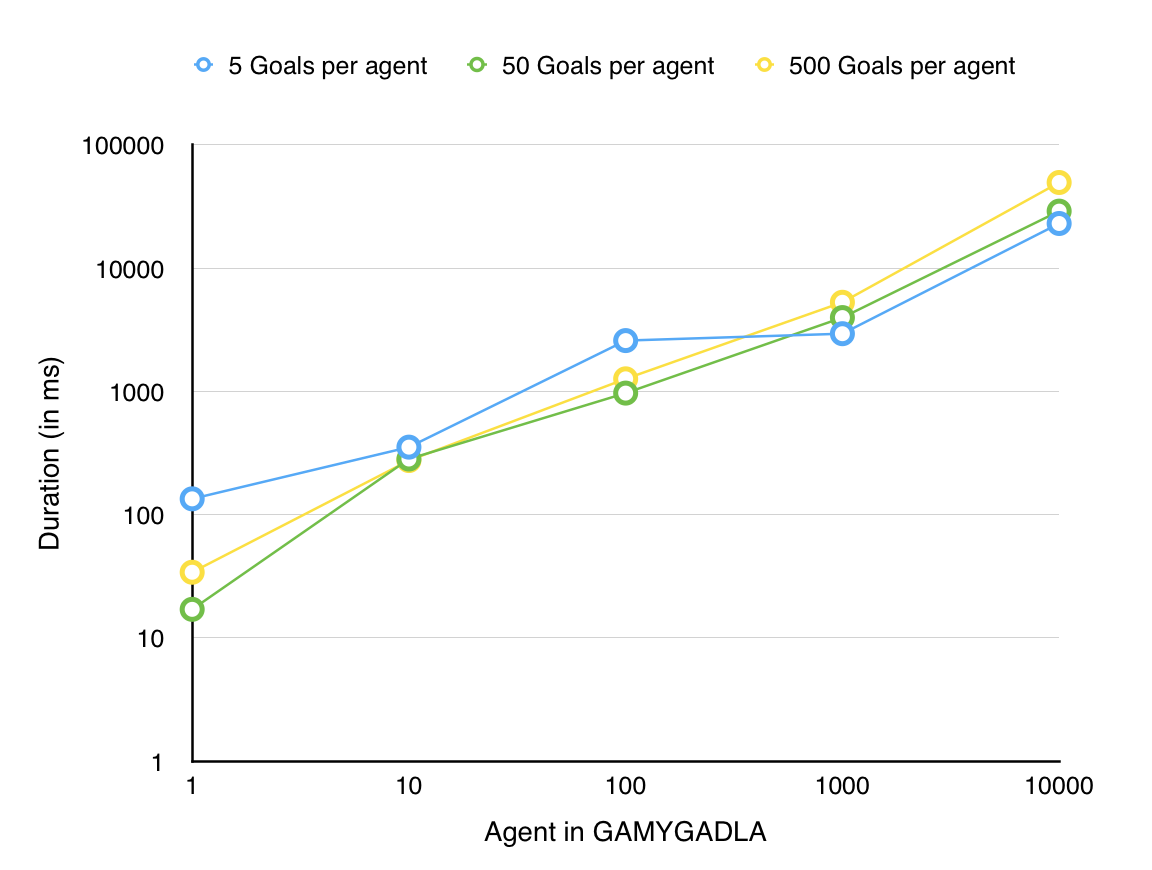
\includegraphics[scale=0.5]{scalability/3.jpg}
  \caption{Scalability, Relation: 100, Belief: 100 and Affected Goals: 100}
  \label{scala:third}
\end{figure}

From these graphs you can see that their is a linear relation between the amount of Agents and the execution time. From this you can conclude that the port of GAMYGDALA is scalable. At least till 10000 Agents, 500 Goals per Agent, 100 Relations, 100 Beliefs and 100 Affected Goals. We think that this is enough, because 1000 Agents with 500 Goals is a really really big system.